\section{Organische Sauerstoffverbindungen -- Alkanole (Alkohole)}
\label{sec:Alkanole}
Alkanole (Alkohole) sind Derivate der Alkane (siehe \vpageref{sec:Alkane}).

Alkanole sind azyklische, aliphatische Kohlenwasserstoffe mit einer
Hydroxylgruppe (OH-Gruppe) im Molekül.
Sie sind Derivate der Alkane.

\begin{description}
	\item[Beispiel:] \ac{C2H5OH} (auch Trinkalkohol, Ethylalkohol oder Weingeist genannt)
\end{description}

\begin{list}{}{}
	\item[Vorüberlegung zur Formel:]~
	\begin{itemize}
		\item Summenformel: \ce{C2H6O}
		\item Lewisschreibweise von \ac{8}: \Lewis{0.24.6,O}
		\item Strukturformel:
			\chemfig{H-!{CH2}-\lewis{26,O}-!{CH2}-H}\hspace{2em}oder\hspace{2em}
%			\textcolor{blue}{
			\chemfig{H-!{CH2}-!{CH2}-\lewis{26,O}-H}
	\end{itemize}
\end{list}

\begin{minipage}{6em}
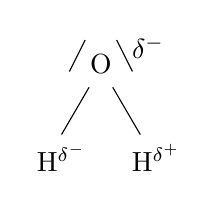
\begin{tikzpicture}[color = {black},scale = 1]
   \draw (1.1,1.8) -- (1.3,2.2);
   \draw (1.9,1.8) -- (1.7,2.2);
   \draw (1,1) -- (1.35,1.6);
   \draw (1.65,1.6) -- (2,1);
   \node[scale = 1] at (1.5,1.9) {O};
   \node[scale = 1] at (2.1,2.1) {$\delta^-$};
   \node[scale = 1] at (1,0.7) {H$^{\delta^-}$};
   \node[scale = 1] at (2.2,0.7) {H$^{\delta^+}$};
\end{tikzpicture}
\end{minipage}
\begin{minipage}{5em}
Wasser
\end{minipage}

Welche ist die richtige Strukturformel? (Die rechte)

Alkohol ist lipophil und hydrophil.

\cVersuch{2}{\acl{C2H5OH} und \acl{11}}
\begin{description}
	\item[Vorüberlegung:] Es entsteht weder eine Base noch eine Säure.
		Wenn das \ac{11} eine Reaktion mit \ac{C2H5OH} zeigt,
		wird die zweite Formel, aufgrund der Ähnlichkeit mit \ac{H2O},
		die Formel für das \ac{C2H5OH} sein.
	\item[Aufbau:] \ac{11} (möglichst ohne Oxidationsschicht) in eine Schale mit
		\ac{C2H5OH} geben. \\
%		(Natrium wird in \ac{C17H36})
	\item[Beobachtung:]~
	\begin{itemize}
		\item Das \acl{11}stückchen löst sich in einer exothermen Reaktion zischend auf.
		\item Es reagiert mit dem \ac{C2H5OH} sehr ähnlich wie mit \ac{H2O}.
	\end{itemize}
	\item[Strukturformel:] \chemfig{H-!{CH2}-!{CH2}-\lewis{26,O}-H}
	\item[Vereinfacht:] \ce{CH3-CH2-\lewis{26,O}H}
	\item[Summenformel:] \ce{C2H6O} oder \acs{C2H5OH}
		\hfil (Merksatz: \textcolor{blue}{H}err \textcolor{blue}{O}ber \textcolor{blue}{5 H}elle
		\textcolor{blue}{2 C}ognak.)
\end{description}

\cVersuch{2}{OH Gruppierung in \acl{C2H5OH} ist anders als in Basen}
\begin{description}
	\item[Aufbau:] 2 Bechergläser,
		Indikatorpapier (Lackmuspapier),
		\ac{NaOH} und \ac{C2H5OH}.
	\item[Beobachtung:]~
	\begin{itemize}
		\item Das Indikatorpapier im \ac{C2H5OH} färbt sich nicht blau,
			wie das in der \ac{NaOH}.
		\item Die OH in Alkanolen ist anders als in Basen.
			Der unterschied liegt in der Bindungsart.
			Bei den Alkanolen besteht eine polare Atombindung zwischen \ac{8} und \ac{1}.
			Bei den Basen hingegen eine Ionenbindung.
	\end{itemize}
	\item[Gleichung:]
		\chemfig{\ce{2H}-!{CH2}-!{CH2}-\lewis{26,O}-H} \chemsign{+} \ce{Na}
		\chemsign{\ce{->}}
		\chemfig{\ce{2H}-!{CH2}-!{CH2}-\lewis{26,O}-Na} \chemsign{+} \ce{H-H} \\[0.8ex]
		\ce{2CH3-CH2-OH + 2Na -> 2CH3-CH2-\lewis{26,O}-Na + H2} \\
		Es entsteht Natriumethanolat und \acl{H2}.
\end{description}

Alkohole reagieren gut mit Alkalimetallen.
Es bilden sich Salze (Alkanolate).

Alkalimetalle + Alkanole \ce{->} Alkanolat/Alkoholat

\ac{NaOH} ist eine Lauge.

Basen (Laugen) sind Stoffe, die in wässriger Lösung oder in der Schmelze in
positiv geladene Metallionen (Kationen)
und negativ geladene Hydroxidionen (Anionen) zerfallen.

\begin{tabular}{p{13em}l}
\ce{NaOH <=> Na^+ + OH^-}		& (Ionenbindung) \\
$\ce{CH3-CH2-\Lewis{26,O}}^{\delta^-}\mathrm{\ce{-H}}^{\delta^+}$
& (polare Atombindung) \\
\end{tabular}

\subsection{Weitere Alkohole}

\begin{description}
	\item[primärer Alkohol:] \chemfig{R-!{CH2}-\textcolor{red}{C}(-[::90]H)(-[::-90]H)-
			\lewis{26,O}-H} \hfil
		(R \entspricht beliebiger Kohlenwasserstoffrest) \\[0.8ex]
		\ac{6}-Atom sitzt an der Hydroxylgruppe und ist nur mit einem weiteren \ac{6}-Atom verbunden.
	\item[sekundärer Alkohol:] \chemfig{R-!{CH2}-
			\textcolor{red}{C}([::90]-[,2]!{CH2}-R)(-[::-90]H)-\lewis{26,O}-H}
	\item[tertiärer  Alkohol:] \chemfig{R-!{CH2}-
			\textcolor{red}{C}([::90]-[,2]!{CH2}-R)([::-90]-[,2]!{CH2}-R)-\lewis{26,O}-H}
\end{description}

\subsection{Mehrwertige Alkohole}
Die Mehrwertigkeit der Alkohole bildet sich durch die Anzahl der Hydroxylgruppen.

\begin{description}
	\item[Beispiele:]~
	\begin{itemize}
		\item 1,2-Ethandiol (Glycol) (zweiwertiger Alkohol) \\[0.5ex]
			\chemfig{H-!{COH}-!{COH}-H}\hspace{3em}bzw.\hspace{3em}\ce{CH2-OH-CH2-OH}
		\item 1,2,3-Propantriol (Glycerol/\ac{C3H8O3}) (dreiwertiger Alkohol) \\[0.5ex]
			\chemfig{H-!{COH}-!{COH}-!{COH}-H} \\[0.8ex]
			Je mehr OH-Gruppen desto süßer.
			\newpage
		\item Hexanhexol (Sorbit) (wird als Süßstoff verwendet) \\[0.5ex]
			\chemfig{H-!{COH}-!{COH}-!{COH}-!{COH}-!{COH}-!{COH}-H}
			\hspace{1em}bzw.\hspace{1em}\ce{CH2OH-(CHOH)4-CH2OH}
	\end{itemize}
\end{description}

\begin{description}
	\item[Erlenmeyer-Regel:] Jedes Kohlenstoffatom bindet nur eine Hydroxylgruppe.
		Ansonsten ist der Stoff instabil, baut sich um oder zerfällt.
\end{description}

\subsection{Funktionelle Gruppe}
Funktionelle Gruppen sind Atome oder Atomgruppen die die Struktur, Eigenschaften
und die chemischen Reaktionen organischer Stoffklassen wesentlich beeinflussen.

Die funktionelle Gruppe der Alkohole ist die
$\mathrm{O}^{\delta^-}\mathrm{H}^{\delta^+}$-Gruppe
(Hydroxylgruppe)

\begin{description}
	\item[Endung:] -ol
\end{description}

\cVersuch{2}{Nachweis mehrerer OH-Gruppen (Hydroxylgruppen) im Molekül}
\begin{description}
	\item[Aufbau:] \ac{C2H5OH}, \ac{C3H8O3}, \ac{H2O}, \ac{CuSO4}, \ac{NaOH},
		2 Bechergläser.
	\item[Durchführung:] \ac{C2H5OH} in das erste Becherglas geben und \ac{C3H8O3} in
		das zweite. Dazu jeweils \ac{H2O}, \ac{CuSO4} und \ac{NaOH} geben.
	\item[Beobachtung:]~
	\begin{itemize}
		\item \ac{C3H8O3} und \ac{C2H5OH} lösen sich in \ac{H2O},
			auch wenn bei \ac{C3H8O3} mit Schlieren.
		\item Auch das \ac{CuSO4} löst sich gut.
		\item Mit dem \ac{NaOH} beginnen sich die Flüssigkeiten blau zu färben,
			wobei das \ac{C3H8O3} mit mehr OH-Gruppen dunkler wird.
	\end{itemize}
\end{description}

\cVersuch{2}{Reaktionsfreudigkeit des \acl{C3H8O3}}
\begin{description}
	\item[Aufbau:] \ac{KMnO4} auf einer feuerfesten Unterlage.
	\item[Durchführung:] \ac{C3H8O3} auf das \ac{KMnO4} geben.
	\item[Beobachtung:] Das \ac{C3H8O3} entreißt dem \ac{KMnO4} in einer stark
		exothermen Reaktion den Sauerstoff (Ähnlichkeit mit \ac{C3H5N3O9})
\end{description}

%\section{Alkanole}
\setcounter{plusplus}{0}
\renewcommand{\longtableheader}{\multicolumn{1}{c}{\textbf{Name}}
& \multicolumn{1}{l}{\textbf{Molekül-}}
& \multicolumn{1}{l}{\textbf{Schmelz-}}
& \multicolumn{1}{l}{\textbf{Siede-}}
& \multicolumn{2}{c}{\textbf{Löslichkeit in}}
& \multicolumn{1}{l}{\textbf{Visko-}}	\\

\multicolumn{1}{c}{\textbf{(Trivialname)}}
& \multicolumn{1}{l}{\textbf{formel}}
& \multicolumn{1}{l}{\textbf{temp. (\si{\degreeCelsius})}}
& \multicolumn{1}{l}{\textbf{temp. (\si{\degreeCelsius})}}
& \multicolumn{1}{c}{\textbf{\acl{H2O},}}
& \multicolumn{1}{c}{\textbf{Benzin}}
& \multicolumn{1}{l}{\textbf{sität}}
\\}
\begin{longtable}{llrrccc}
	\longtableheader
	\endfirsthead
	\longtableheader
	\endhead
	\caption{Die homologe Reihe der Alkanole}
	\endlastfoot
	\multicolumn{7}{r}{\longtableendfoot} \\
	\endfoot

	\tableprintACSandACL{CH3OH} 	& $-97$		& 65	& & & \stepcounter{plusplus} \\
	(Methylalkohol)		& & & & & & \stepcounter{plusplus} \\
	\tableprintACSandACL{C2H5OH}	& $-114$	& 78	& & & \stepcounter{plusplus} \\
	(Ethylalkohol)		& & & & & & \stepcounter{plusplus} \\
	\tableprintACSandACL{C3H7OH}	& $-126$	& 97	& & & \stepcounter{plusplus} \\
	(Propylalkohol)		& & & & & & \stepcounter{plusplus} \\
	\tableprintACSandACL{C4H9OH}	& $-90$		& 118	& & & \stepcounter{plusplus} \\
	(Butylalkohol)		& & & & & & \stepcounter{plusplus} \\
	\tableprintACSandACL{C5H11OH}	& $-78$		& 138	& & & \stepcounter{plusplus} \\
	(Pentylalkohol)		& & & & & & \stepcounter{plusplus} \\
	\tableprintACSandACL{C6H13OH}	& $-47$		& 158	& & & \stepcounter{plusplus} \\
	(Hexylalkohol)		& & & & & & \stepcounter{plusplus} \\
	\tableprintACSandACL{C12H25OH}	& 26		& 256	& & & \stepcounter{plusplus} \\
	(Laurylalkohol)		& & & & & & \stepcounter{plusplus} \\
	\tableprintACSandACL{C16H33OH}	& 50		& 344	& & & \stepcounter{plusplus} \\
	(Cetylalkohol)		& & & &
	\multirow{-\value{plusplus}}{*}{\rotatebox{-90}{$\autorightarrow{nimmt zu}{}$}} &
	\multirow{-\value{plusplus}}{*}{\rotatebox{-90}{$\autorightarrow{nimmt zu}{}$}} &
	\multirow{-\value{plusplus}}{*}{\rotatebox{-90}{$\autorightarrow{nimmt zu}{}$}}
	\stepcounter{plusplus} \\
\end{longtable}

Unter anderem die Siedetemperatur der Alkanole ist viel höher als die der Alkane.
Dies liegt an der Funktionellen Gruppe.

$\mathrm{C_nH_{2n+1}OH}$

%Alkanole bilden eine homologe Reihe.

\cVersuch{2}{\acl{C4H9OH} und \acl{H2O}}
\begin{description}
	\item[Aufbau und Durchführung:] In ein Reagenzglas \ac{C4H9OH} und \ac{H2O} geben.
	\item[Beobachtung:] Die Flüssigkeiten bilden eine Emulsion,
		die sich ganz schnell wieder entmischen.
	\item[Erklärung:]~
	\begin{itemize}
		\item Je länger die Kette, desto schwerer wasserlöslich.
		\item OH-Gruppe sorgt für eine Verbesserung der Wasserlöslichkeit (hydrophil).
		\item Der Kohlenwasserstoff sorgt für eine Verschlechterung der
			Wasserlöslichkeit (hydrophob).
	\end{itemize}
\end{description}

\cVersuch{2}{\acl{C5H11OH} und \acl{C6H6}}
\begin{description}
	\item[Aufbau und Durchführung:] In ein Reagenzglas \ac{C5H11OH} und \ac{C6H6} geben.
	\item[Beobachtung:] Die Flüssigkeiten vermischen sich sehr gut.
	\item[Erklärung:] Langkettige Alkohole werden immer Benzinähnlicher.
\end{description}

\cVersuch{2}{\acl{C2H5OH} und \acl{C5H11OH}}
\begin{description}
	\item[Aufbau und Durchführung:] \ac{C2H5OH} und \ac{C5H11OH} in jeweils eine Abdampfschale geben
		und anzünden.
	\item[Beobachtung bei \ac{C2H5OH}:] Lässt sich mit einem Holzstäbchen entzünden.
		Brennt mit gelber Flamme.
	\item[Beobachtung bei \ac{C5H11OH}:] Lässt sich nicht mit einem Holzstäbchen entzünden.
		Nach erhitzen mit dem Bunsenbrenner brennt es mit kräftiger orangefarbener Flamme.
	\item[Erklärung:] Je länger die Kohlenstoffketten werden,
		desto orangener wird die Flamme und desto schwerer sind diese Stoffe zu entzünden.
	\item[Gleichung:] Alle Alkanole verbrennen zu \ac{CO2} und \ac{H2O}.
	\begin{align}
		\ce{C3H7OH + 4 1/2O2}	& \ce{-> 3CO2 + 4H2O} \\
		\ce{2C3H7OH + 9O2}	& \ce{-> 6CO2 + 8H2O}
	\end{align}
\end{description}

\cVersuch{2}{\acl{C6H12O6} und \acl{H2SO4}}
\begin{description}
	\item[Aufbau und Durchführung:] In ein Becherglas \ac{C6H12O6},
		auch als Traubenzucker bezeichnet, und \ac{H2SO4} geben.
	\item[Beobachtung:]~
	\begin{itemize}
		\item Zucker wird gelb, braun und dann Schwarz.
			Es entsteht Hitze, Qualm und ein stechender Geruch.
			Das entstehende \ac{CO2} sorgt für eine Volumenzunahme
			von \ac{C6H12O6}.
		\item Es entsteht Zuckerkohle und \ac{CO2}.
	\end{itemize}
	\item[Erklärung:] Die \ac{H2SO4} entzieht dem Zucker das \ac{H2O}.
\end{description}

\cVersuch{2}{\acl{C2H5OH} und \acl{H2SO4}}
\begin{description}
	\item[Aufbau und Durchführung:] \ac{C2H5OH} und \ac{H2SO4} in ein Reagenzglas geben
		und etwas erhitzen. \\
		\begin{figurewrapper}\vspace{-1em}
			\includegraphics[width=0.15\hsize]{files/pst-labo/C2H5OH+H2SO4-pics}
			\captionof{figure}{\acl{C2H5OH} und \acl{H2SO4}}
		\end{figurewrapper}\vspace{-1em}
	\item[Beobachtung:] Es kommt zu einer exothermen Reaktion wenn \ac{C2H5OH} und \ac{H2SO4}
		zusammen kommen. Das Reagenzglas wird warm und die Flüssigkeit wird Gelblich.
	\item[Erklärung:] Langkettige Alkohole werden immer Benzinähnlicher.
	\item[Gleichung bei einer Temperatur kleiner \textbf{\SI[detect-weight]{140}{\degreeCelsius}}:]
		Es entsteht \ac{C4H10O}. \\[0.5em]
		\ce{CH3-CH2-\lewis{26,O}-H + H-\lewis{26,O}-CH2-CH3
			->[\text{c \acs{H2SO4}}] H2O + CH3-CH2-\lewis{26,O}-CH2-CH3} \\
		Alkohol + Säure \ce{->} Ether + \ac{H2O} \\
		Substitution und Dehydratisierung (wegen \ac{H2O} Abspaltung) \\
		Stoffe mit folgendem Aufbau nennt man Ether. \\[0.3em]
		\begin{minipage}{7em}
			\ce{R1-\lewis{26,O}-R2}
		\end{minipage}
		\begin{minipage}{5em}
			$\mathrm{R_1 = R_2}$ \\
			$\mathrm{R_1 \neq R_2}$
		\end{minipage}\hfill
		\begin{minipage}{25em}
			Innermolekulare Gruppe: Der \ac{6} ist ins Molekül eingebaut.
		\end{minipage}
	\item[Gleichung bei einer Temperatur über \textbf{\SI[detect-weight]{140}{\degreeCelsius}}:]
		Es entsteht \ac{C2H4} und \ac{C2H4}. \\[0.5em]
		\chemfig{H-!{CH2}-C(-[::90]H)(-[::-90]\textcolor{red}{H})-\textcolor{red}{\lewis{26,O}-H}}
		\chemsign{\ce{->[\text{c \acs{H2SO4}}]}} \textcolor{red}{\ce{H2O}} \chemsign{+}
		\chemfig{C(-[::135]H)(-[::-135]H)=C(-[::45]H)(-[::-45]H)} \\[0.5em]
		Aus Alkohol wird Alken und \ac{H2O}
\end{description}

\subsection{Eliminierung}
Eine Eliminierung ist eine chemische Reaktion,
bei der Stoffe oder Stoffgruppen aus einer Verbindung abgespalten werden,
unter Errichtung einer Mehrfachbindung.

\donkeybridge{zur Eliminierung: \enquote{Aus 1 mach 2}}
{

\centering\hspace{-2em}
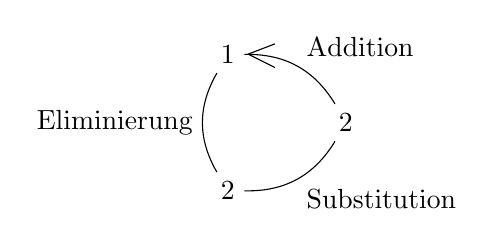
\begin{tikzpicture}[auto,bend right]
	\node (a) at (0:1) {2};
	\draw (0.1,1) -- (-0.24,0.87) -- (0.1,0.7);
	\node (b) at (120:1) {1};
	\node (c) at (240:1) {2};
	\draw (a) to node [swap] {Addition} (b)
		(b) to node [swap] {Eliminierung} (c)
		(c) to node [swap] {Substitution} (a);
\end{tikzpicture}

}

\subsection{Typische Reaktionen der Alkohole}
\begin{itemize}
	\item Verbrennen zu \ac{CO2} und \ac{H2O}.
	\item Reagieren mit Alkalimetallen zu Alkoholaten (Alkoholaten).
	\item Bei Entzug von \ac{H2O} entsteht Ether.
\end{itemize}

\subsection{Reaktionsgleichungen zu Verbrennungen}
Verbrennung von \ac{CH3OH} und \ac{C2H5OH}.
\begin{align}
	\ce{2CH3OH + 3O2}	& \ce{-> 6CO2 + 8H2O} \\
	\ce{C2H5HO + 3O2}	& \ce{-> CO2 + 2H2O}
\end{align}

\subsection{Reaktion von \acl{CH3OH}}
\ac{CH3OH} reagiert bei Temperaturen unter \SI[detect-weight]{140}{\degreeCelsius}.

\ce{CH3-\lewis{26,O}-H + H-\lewis{26,O}-CH3 ->[\text{c \acs{H2SO4}}] H2O + CH3-\lewis{26,O}-CH3}

Es entsteht \ac{H2O} und \ac{C4H10O}. Diese Reaktion ist eine Substitution oder
genauer eine Dehydratisierung.

\subsection{Reaktion von \acl{C3H7OH}}
\ac{C3H7OH} reagiert bei Temperaturen über \SI[detect-weight]{140}{\degreeCelsius}.

\chemfig{H-!{CH2}-!{CH2}-!{CH2}-\lewis{26,O}-H} \chemsign{\ce{->}}
\ce{H2O} \chemsign{+}
\chemfig{C(-[::135]H)(-[::-135]H)=C(-[::90]H)-\lewis{26,O}-H}

Es entsteht \ac{H2O} und \ac{C3H6}. Diese Reaktion ist eine Eliminierung oder
genauer eine Rehydratisierung.

\subsection{Übersicht der funktionelle Gruppen}

\renewcommand{\longtableheader}{\multicolumn{1}{l}{\textbf{Funktionelle und intermediäre Gruppe}}
& \multicolumn{1}{l}{\textbf{Name}}
& \multicolumn{1}{l}{\textbf{Endungen}}
\\
}
\begin{longtable}{lll}
	\longtableheader
	\endfirsthead
	\longtableheader
	\endhead
	\caption{Übersicht der funktionelle Gruppen}
	\endlastfoot
	\multicolumn{3}{r}{\longtableendfoot} \\
	\endfoot

	$\mathrm{R_1-\lewis{26,O}-R_2}$\footnote{keine echte funktionelle Gruppen, sondern eine besondere
		Verbindung.} & & -ether \\
	\chemfig{-\lewis{26,O}-H}	& Hydroxy(l)gruppe		& -ol \\[1em]
	\chemfig{-C(=[::45]\lewis{02,O})(-[::-45]H)}	& Aldehydgruppe		& -al \\[2.5em]
	\chemfig{-C(=[::90]\lewis{13,O})-}				& Ketogruppe		& -on \\
\end{longtable}

Primäre Alkohole lassen sich zu Aldehyden, sekundäre zu Ketonen oxidieren.
